% APORTE TERCER AVANCE (CIERRE) - VELEZ VINCES JOSTIN GUSTAVO (CI: 1316917838)
% Incluye: Paso 5c (Tabla de las 8 Perspectivas de Contexto de Pohl: 24 preguntas y 16 requisitos emergentes), Paso 5d (Mapa Conceptual Figura 1) y Conclusión 3

\subsubsection{c) Análisis Exhaustivo de las Ocho Perspectivas de Contexto de Pohl Aplicadas al PFC}
Conforme al Paso 5c de la Guía de Práctica y al marco teórico de Klaus Pohl (2025) \cite{pohl2025}, en la Tabla \ref{tab:ocho_perspectivas} se evalúan las ocho perspectivas de contexto sobre el sistema del PFC, formulando para cada una (a) \textbf{tres preguntas clave de indagación} (24 preguntas en total) y (b) \textbf{dos requisitos o restricciones concretas que emergen} de dicho análisis (16 requisitos/restricciones emergentes en total).

\begin{table}[htbp]
\centering
\scriptsize
\caption{Aplicación de las Ocho Perspectivas de Contexto de Pohl (2025) \cite{pohl2025} al Sistema del PFC}
\label{tab:ocho_perspectivas}
\begin{tabularx}{\textwidth}{l Y Y}
\toprule
\textbf{Perspectiva de Contexto \cite{pohl2025}} & \textbf{(a) Tres Preguntas Clave de Elicitación Contextual} & \textbf{(b) Dos Requisitos / Restricciones que Emergen para el PFC} \\
\midrule
\textbf{1. Perspectiva de Sujeto (Datos y Dominio)} & 
1. ¿Qué atributos técnicos definen la compatibilidad eléctrica entre dos componentes (voltaje nominal, amperaje, curva de disparo, calibre AWG, número de polos)? \newline
2. ¿Cómo se estructuran las relaciones de equivalencia e intercambiabilidad en el catálogo de productos? \newline
3. ¿Qué volumen histórico de facturas y movimientos de kardex debe almacenarse activamente? & 
\textbf{Emergente 1.1:} El esquema PostgreSQL deberá almacenar especificaciones técnicas estructuradas en un campo indexado \texttt{JSONB} por producto (tensión, corriente, norma IEC/NEMA) para alimentar el prompt de Groq. \newline
\textbf{Emergente 1.2:} Toda sugerencia de la IA estará restringida únicamente a productos con \texttt{stock\_actual > 0} en la bodega local. \\
\midrule
\textbf{2. Perspectiva de Uso (Actores y Flujos)} & 
1. ¿Cuál es el nivel de alfabetización digital y de conocimientos en electricidad de los cajeros actuales del local en Quevedo? \newline
2. ¿Con qué frecuencia un cliente pide asesoría técnica frente a una compra directa por lista? \newline
3. ¿Qué tareas repetitivas generan mayor fatiga o errores de digitación en el turno diario? & 
\textbf{Emergente 2.1:} La interfaz de caja operará mediante flujo completo de teclado (atajos F1--F12) y foco automático en el campo de código de barras (ref. REQ-03). \newline
\textbf{Emergente 2.2:} Las 3 recomendaciones de la IA mostrarán en lenguaje claro por qué el ítem es compatible y cuál es su diferencia de precio. \\
\midrule
\textbf{3. Perspectiva de Entorno TI (Infraestructura)} & 
1. ¿Qué sistemas operativos, navegadores y servidores utiliza actualmente el almacén eléctrico? \newline
2. ¿Qué ocurre con la operación del punto de venta si se cae el enlace de internet con Groq Cloud o con el SRI? \newline
3. ¿Qué periféricos físicos están conectados en los puestos de caja? & 
\textbf{Emergente 3.1:} El sistema implementará un mecanismo de \textit{Circuit Breaker}: si Groq supera los $3.0\text{ s}$ de latencia, conmutará automáticamente a una consulta SQL local de productos de la misma subcategoría en $\le 200\text{ ms}$ (ref. REQ-10). \newline
\textbf{Emergente 3.2:} Compatibilidad nativa con escáneres USB HID e impresoras térmicas ESC/POS de 80 mm (ref. REQ-13). \\
\midrule
\textbf{4. Perspectiva de Desarrollo (Entorno de Ingeniería)} & 
1. ¿Qué stack tecnológico domina el equipo de ingeniería (José, Jostin y Jeanpierre) para garantizar entregas de alta calidad en el semestre? \newline
2. ¿Cómo se gestionará el control de versiones, despliegue reproducible y pruebas automatizadas? \newline
3. ¿Qué herramientas de análisis y modelado se exigen en el entorno académico de la UTEQ? & 
\textbf{Emergente 4.1:} Restricción de construcción en Python 3.12 con framework Django, base de datos PostgreSQL 16 y contenedorización mediante Docker sobre Linux (ref. REQ-15). \newline
\textbf{Emergente 4.2:} Gestión de código y documentación técnica LaTeX en repositorio Git/GitHub con trazabilidad de commits por integrante. \\
\midrule
\textbf{5. Perspectiva Física (Ambiente Operativo)} & 
1. ¿Cuáles son las condiciones de iluminación, reflejo solar, polvo y ruido ambiental en el mostrador de atención del local eléctrico? \newline
2. ¿De cuánto espacio físico dispone el cajero en el mostrador para ubicar monitor, teclado y lector óptico? \newline
3. ¿Existen fluctuaciones o cortes de energía eléctrica frecuentes en la zona comercial de Quevedo? & 
\textbf{Emergente 5.1:} La interfaz gráfica aplicará alto contraste visual (WCAG 2.1 nivel AA) y tipografía mínima de 14 px para facilitar la lectura rápida bajo iluminación fluorescente intensa (ref. REQ-12). \newline
\textbf{Emergente 5.2:} El servidor local PostgreSQL contará con respaldo de energía UPS y transacciones ACID para evitar corrupción de datos ante apagones. \\
\midrule
\textbf{6. Perspectiva Social y Cultural} & 
1. ¿Existe temor o resistencia del personal de caja a ser reemplazado o evaluado negativamente por la introducción de la IA? \newline
2. ¿Cómo perciben los maestros electricistas de Quevedo las recomendaciones generadas por una computadora? \newline
3. ¿Qué terminología coloquial local utilizan los clientes para pedir materiales eléctricos (ej. ``breaker'', ``taipe'', ``boquilla'')? & 
\textbf{Emergente 6.1:} El prompt del sistema en Groq incluirá un diccionario de sinónimos y jerga ferretera ecuatoriana (ej. mapear ``breaker'' a ``interruptor termomagnético'' y ``taipe'' a ``cinta aislante vinílica''). \newline
\textbf{Emergente 6.2:} La IA fungirá como copiloto de apoyo al cajero (quien tiene la decisión final de venta), no como sustituto autónomo. \\
\midrule
\textbf{7. Perspectiva Legal y Regulatoria} & 
1. ¿Qué normativas tributarias rigen la emisión y transmisión de comprobantes de venta en el Ecuador en 2026? \newline
2. ¿Cómo afecta la Ley Orgánica de Protección de Datos Personales (LOPDP) al almacenamiento de datos de clientes y al envío de prompts a la nube? \newline
3. ¿Qué normas técnicas eléctricas (INEN / NEC) deben respetarse al sugerir un componente sustituto? & 
\textbf{Emergente 7.1:} Cumplimiento estricto del esquema XSD v2.1.0 de Facturación Electrónica del SRI con firma electrónica PKCS\#12 y tarifa IVA del 15\% (ref. REQ-05, REQ-07). \newline
\textbf{Emergente 7.2:} Prohibición de enviar datos personales identificables (cédula, RUC, nombres o correos de clientes) hacia la API externa de Groq Cloud (cumplimiento LOPDP). \\
\midrule
\textbf{8. Perspectiva Económica y Organizacional} & 
1. ¿Cuál es el presupuesto máximo mensual que el propietario puede destinar al consumo de tokens de API de Inteligencia Artificial y servidores? \newline
2. ¿Qué retorno de inversión (ROI) y reducción de costos operativos espera alcanzar la gerencia en el corto plazo? \newline
3. ¿Cómo impacta el sistema en el proceso de arqueo y cierre de caja diario del negocio? & 
\textbf{Emergente 8.1:} Optimización de consumo de tokens mediante caché en memoria (Redis/Django Cache) para consultas técnicas repetidas sobre un mismo código SKU durante el día. \newline
\textbf{Emergente 8.2:} Generación automática del reporte de cuadre de caja diario desglosado por forma de pago y ventas originadas por sugerencias de la IA en $\le 2.0\text{ s}$. \\
\bottomrule
\end{tabularx}
\end{table}

\subsubsection{d) Mapa Conceptual Integrador de la Unidad I (Figura 1)}
En la Figura \ref{fig:mapa_conceptual} se presenta el mapa conceptual integrador desarrollado por el equipo, el cual articula los cuatro ejes temáticos de la Unidad I (Fundamentos de IR, Taxonomía y Propiedades de Calidad, Contexto y 8 Perspectivas, y Proceso/Framework de IR) e incorpora explícitamente cuatro vínculos cruzados semánticos y su aterrizaje directo en la Plataforma POS con IA Groq del PFC (ver Anexo B para evidencias complementarias).

\begin{figure}[htbp]
\centering
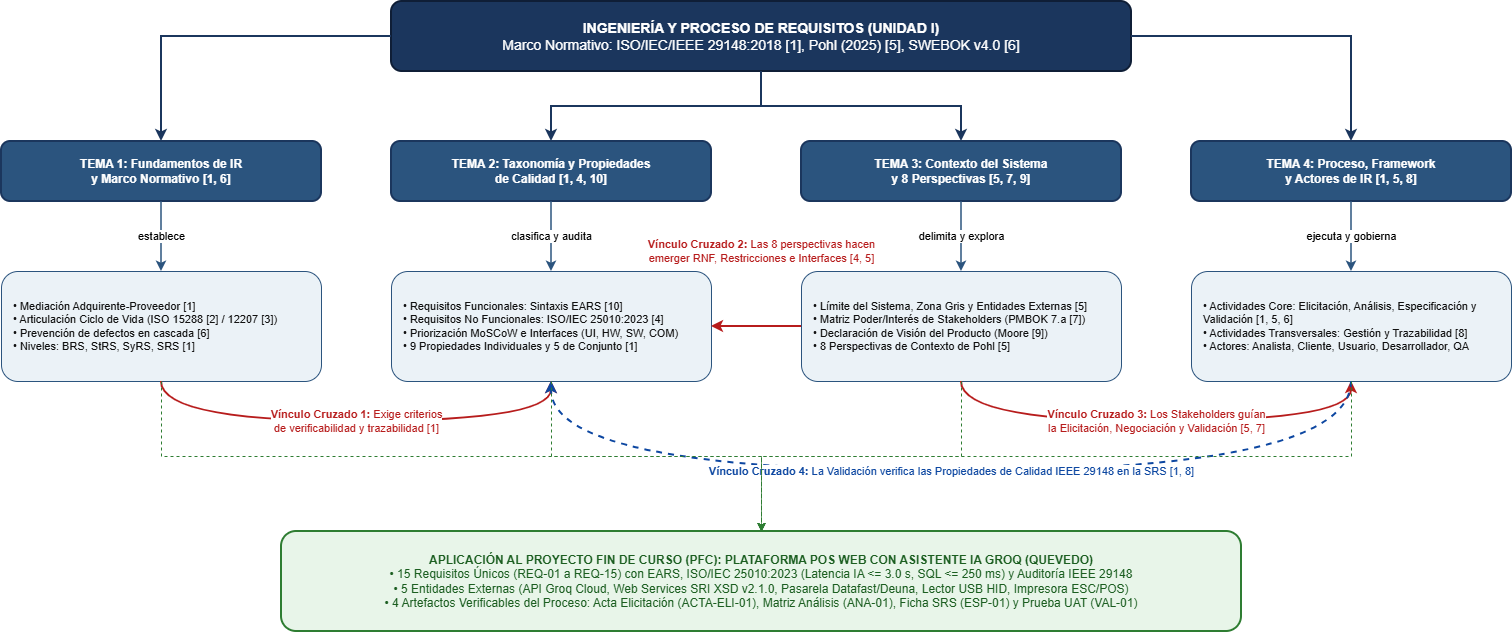
\includegraphics[width=0.98\textwidth]{figura/mapa_conceptual.png}
\caption{Mapa Conceptual Integrador de los Cuatro Temas de la Unidad I con Vínculos Cruzados y Aplicación al PFC.}
\label{fig:mapa_conceptual}
\end{figure}


\section*{Conclusión Individual --- Jostin Gustavo Vélez Vinces}
\begin{itemize}
\item \textbf{Conclusión 3 --- Vélez Vinces Jostin Gustavo (Sobre el Límite del Sistema y las Ocho Perspectivas de Contexto de Pohl):} \\
    \textbf{(1) Afirmación:} Analizar de forma sistemática el entorno donde operará el software mediante perspectivas multidimensionales permite descubrir restricciones físicas, sociales y legales ocultas que jamás emergerían en una entrevista superficial. \textbf{(2) Evidencia con cita:} Según Klaus Pohl (2025) \cite{pohl2025} y el sílabo IREB CPRE v3.1 \cite{ireb2023}, el contexto del sistema debe explorarse a través de ocho perspectivas complementarias (sujeto, uso, TI, desarrollo, física, social, legal y económica) para delimitar con precisión la zona gris y las interfaces externas. \textbf{(3) Implicación para el PFC y la profesión:} Aplicar las ocho perspectivas al contexto comercial de Quevedo nos permitió identificar requisitos decisivos para el PFC, tales como incluir un diccionario de jerga eléctrica ecuatoriana (``breaker'', ``taipe'') en el prompt de la IA, restringir el envío de datos personales a la nube por mandato de la LOPDP y exigir cumplimiento estricto con el esquema XML XSD v2.1.0 del SRI.

    \end{itemize}
